\section{Closed-Loop Simulations}
In this section the MPC's determined in \cref{sec:uncon_MPC}, \ref{sec:in_con_MPC} and \ref{sec:in_out_con_MPC} will be simulated on both the linear models and the non-linear models.\\
The reference signal is modelled as shown in \cref{tab:CL_sim_ref}. The system is initialized from steady state, where $u=\begin{bmatrix} 300 & 300\end{bmatrix}^T$. The disturbance is set be stochastic variable which follows a normal distribution given by: $d=N(250,\sqrt{10})$. The measurement noise is modelled as normal distributed according to $v_k=N(0,\sqrt{20})$.
\begin{table}[H]. 
    \centering
    \begin{tabular}{|ccc|} \hline
         Time [min] & $\Delta r_1$ [m] & $\Delta r_2$ [m] \\ \hline
         0 & 0 & 0\\
         10 & 10 & 10\\
         20 & 20 & -10 \\\hline
    \end{tabular}
    \caption{Reference signal}
    \label{tab:CL_sim_ref}
\end{table}
For all simulations, the overall concept is done by the MPC predicts 2*N (where $N=40$) number of inputs ahead. Then the first coming two rows in the prediction (due to the fact that we have two inputs) is saved as the input for the k\textsuperscript{th} iteration. This is used in both the linear model (as a deviation variable) and in the non-linear model (as absolute value). Then the non-linear and linear states is determined and finally the measurement is done. The measurement are then used as inputs to the Kalman filter in order to estimate the states, and filter out measurement noise. 
\subsection{Design of Unconstrained MPC - Point 1, 2 \& 3}
\label{sec:uncon_MPC}
The objective of the MPC is to be minimized, which can be described as a least square problem (for unconstrained MPC), which for a discrete time state space is given by
\begin{equation}
    \underset{x\in R^n}{f(x)}=\frac{1}{2}=\norm{Ax-b}_2^2=\frac{1}{2}\,x^TA^TAx-(A^Tb)^Tx+\frac{1}{2}\,b^Tb
\end{equation}
Where the expression can be rewritten in according to $H=A^TA$, $g=-A^Tb$ and $\rho=\frac{1}{2}\,b^Tb$. The unconstrained optimization problem is defined for the vector case as seen below
\begin{equation}
    \underset{x\in R^n}{f(x)}=\frac{1}{2}\,x^THx+g^Tx
    \label{eq:uncon_f}
\end{equation}
Where $\nabla f(x)=Hx+g=0$ and $\nabla^2f(x)=H\geq 0$ is necessary and sufficient optimality conditions. $H$ is positive definite and the solution is unique.\\
The MPC aims to find e.g. an input value, for which a predetermined function has a minimum. The minimization is determine based on weights $S$ and $Q$ (which is the tuning parameters).\\
The MPC is designed for the linear discrete time model determined in \cref{sec:Dis_LTI}. It is desired that the control input variation and the error on the output should be minimized, which yields the following least square problem.
\begin{equation}
    \text{min}\quad \phi=\frac{1}{2}\, \overset{N}{\underset{k=0}{\sum}}\norm{z(k)-r_k}_{Q_z}^2+\frac{1}{2}\, \overset{N-1}{\underset{k=0}{\sum}}\norm{\Delta u_k}_S^2
    \label{eq:MPC_uncon_lsq}
\end{equation}
Where $N$ is the prediction horizon, $z(k)$ is the output vector (which can be determine in according to \cref{eq:uncon_z}), $r(k)$ is the reference vector, $Q_z$ and $S$ is the weight matrices and $\Delta U_k=U_k-U_{k-1}$.\\
First the minimized output (1\textsuperscript{st} part of the equation) is analyzed.
\begin{equation}
    Z=\phi\,x_0+\Gamma\,U+\Gamma_d\,D
    \label{eq:uncon_z}  
\end{equation}
Notice that since the disturbance is unknown, $D$ is unknown. Hence, the matrix $\Gamma_d$ is not used in the simulation. Each element is determined as
\begin{equation}
    \begin{gathered}
        Z=\begin{bmatrix}
            z_1\\
            z_2\\
            z_3\\
            \vdots\\
            z_N
        \end{bmatrix} \quad
        \phi=\begin{bmatrix}
            CA\\
            CA^2\\
            CA^3\\
            \vdots\\
            CA^N
        \end{bmatrix} \quad
            \Gamma=\begin{bmatrix}
            H_1 & 0 & 0 & \dots & 0\\
            H_2 & H_1 & 0 & \dots & 0\\
            H_3 & H_2 & H_1 & \dots & 0\\
            \vdots & \vdots & \vdots & \ddots & \vdots\\
            H_N & H_{N-1} & H_{N-2} & \dots & H_1
        \end{bmatrix} \\
        H_N=CA^{i-1}B
    \end{gathered}
    \label{eq:uncon_design}
\end{equation}
The expression of $z(k)$ is now substituted into the first part of the least square problem (containing the output).
\begin{equation}
    \phi_z=\frac{1}{2}\norm{\phi\,x_0+\Gamma\,U-R}_{Q_z}^2
\end{equation}
It is desired to have the form seen in \cref{eq:uncon_f}, why the above expression is rewritten by using linear algebra, which yields
\begin{equation}
    \phi_z=\frac{1}{2}U^T\underbrace{(\Gamma^TQ_z\Gamma)}_HU+{\underbrace{(-\Gamma^TQ_zK)}_{g}}^TU+\underbrace{\frac{1}{2}K^TQ_zK}_\rho\qquad , \qquad K=R-\phi x_0     
\end{equation}
Now the minimized control input variation (2\textsuperscript{nd} part) is analyzed.
\begin{equation}
    \phi_{\Delta_u}=\frac{1}{2}\,U^TH_sU+(M_{u1}\,u_{-1})^TU
\end{equation}
Where each element matrix is determined as
\begin{equation*}
    U=\begin{bmatrix}
    u_1\\u_2\\u_3\\\vdots\\u_N
    \end{bmatrix}\qquad
    H_s=\begin{bmatrix}
    2S & -S & 0 & \dots & 0\\
    -S & 2S & -S & \dots & 0\\
    0 & -S & 2S & \dots & 0\\
    \vdots & \vdots & \vdots & \ddots & \vdots\\
    0 & 0 & 0 & -S & S
    \end{bmatrix}\qquad
    M_{u1}=-\begin{bmatrix}
    S \\ 0 \\ 0 \\ \vdots \\ 0
    \end{bmatrix}
\end{equation*}
Now the two optimizations objects is added together, so the complete minimization is
\begin{equation}
    \label{eq:MPC_obj}
    \underset{U}{min}\,\phi=\phi_z+\phi_{\Delta u}=\frac{1}{2}U^THU+g^TU
\end{equation}
Where
\begin{equation}
    \label{eq:M_mat_MPC}
    \begin{gathered}
        H=H_z+H_s=\Gamma^TQ_z\Gamma+H_s\\
        g=M_{x0}\,x_0+M_R\,R+M_{u1}\,u_{-1}\\
        M_{x0} = \Gamma^TQ_z\phi \quad M_R=-\Gamma^TQ_z
    \end{gathered}
\end{equation}
\\\\
The implementation in \textit{MatLab} is carried out through three functions. Prior to the simulation, the MPC design i carried out (see \cref{app:MPC_design}) where, $H$, $H_s$ and $g$ is determined. In order to do this, the function calls a seperate function (see \cref{app:MPC_Constants}) where $\phi$ and $\Gamma$ is determined. Finally, the qpsolver is called. Notice, that since the simulation is unconstrained, the only inputs are $H$, $H_s$ and $g$ (see \cref{app:Uncon_MPC})
\subsection{Input Constrained MPC - Closed Loop Simulation}
In this section the input constrained MPC is simulated on both the linear and non-linear system. For this simulation, the tuning is set to $Q=100$ and $S=0.01$. The constraints is set to 
\begin{equation}
    u_{min}=0\qquad u_{max}=450\qquad \Delta u_{min}=-10\qquad \Delta u_{max}=10
\end{equation}
It should be noticed that the values shown in the plot is absolute values.
\begin{figure}[H]
    \centering
    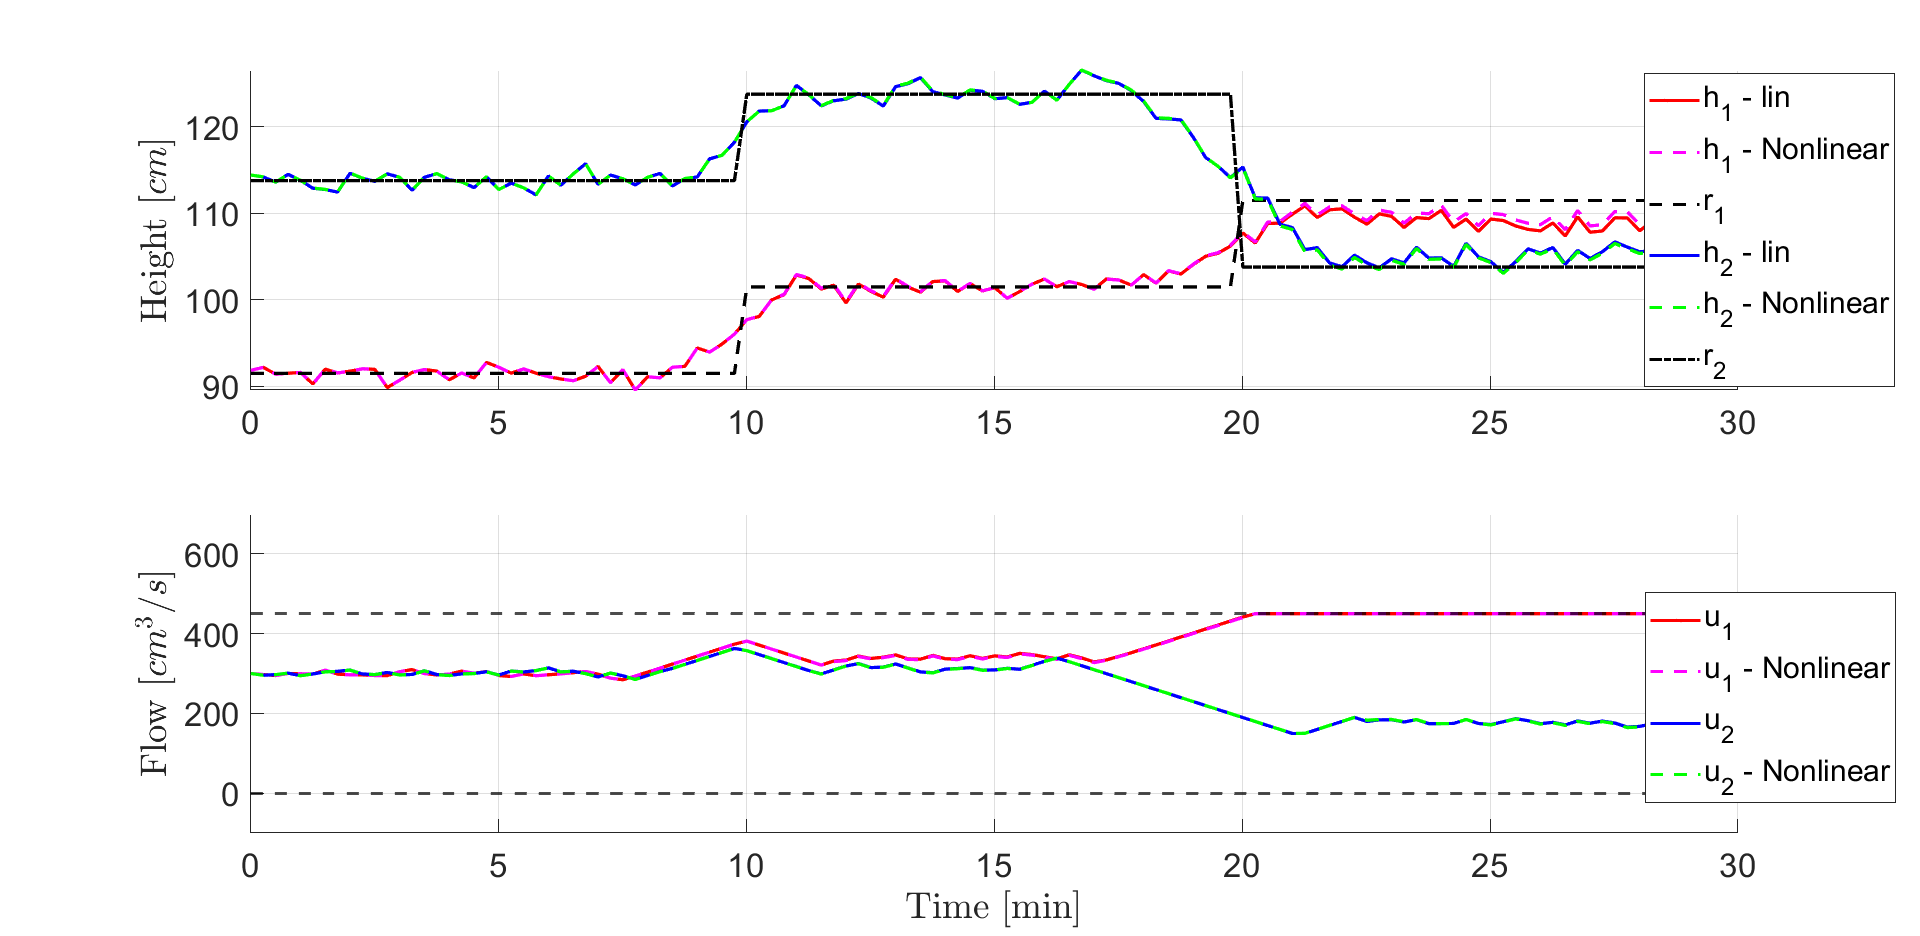
\includegraphics[width=1\textwidth]{Figures/Pr10.2_Input_con_MPC.png}
    \caption{Input constrained MPC - Simulation on linear and non-linear model}
    %\label{fig:Kalman_stoc_state_step}
\end{figure}
As for the unconstrained MPC, the deviation between the linear and the non-linear system is very small. In the case of input constrained MPC, the settling time (in case of step changes in the reference) is longer which is intuitive when the inputs are constrained. It is also seen that the MPC try to regulate earlier (in relation to at which time the reference occurs). In case the constraints on $\Delta u$ was lower, the regulation will begin earlier.
It can be seen that the input 1 is reaching its maximum limit, which causes the reference in tank 1 to be unreachable (however very close). 
\subsection{Input Constrained and Soft Output Constrained MPC - Closed Loop Simulation}
In this section the hard input and soft output constrained MPC is simulated on both the linear and non-linear system. For this simulation, the tuning is set as:
\begin{equation}
    \begin{gathered}
        W_z=100 \quad W_u=0 \quad W_{du}=0\\
        W_{t1}=10000 \quad W_{t2}=10000 \quad W_{s1}=10000 \quad W_{s2}=10000
    \end{gathered}
\end{equation}
The constraints is set to 
\begin{equation}
    u_{min}=0\quad u_{max}=450\quad \Delta u_{min}=-10\quad \Delta u_{max}=10 \quad Z_{min} = \begin{bmatrix} 85 \\ 105 \end{bmatrix} \quad Z_{max} = \begin{bmatrix} 110 \\ 120 \end{bmatrix}
\end{equation}
It should be noticed that the values shown in the plot is absolute values.
\begin{figure}[H]
    \centering
    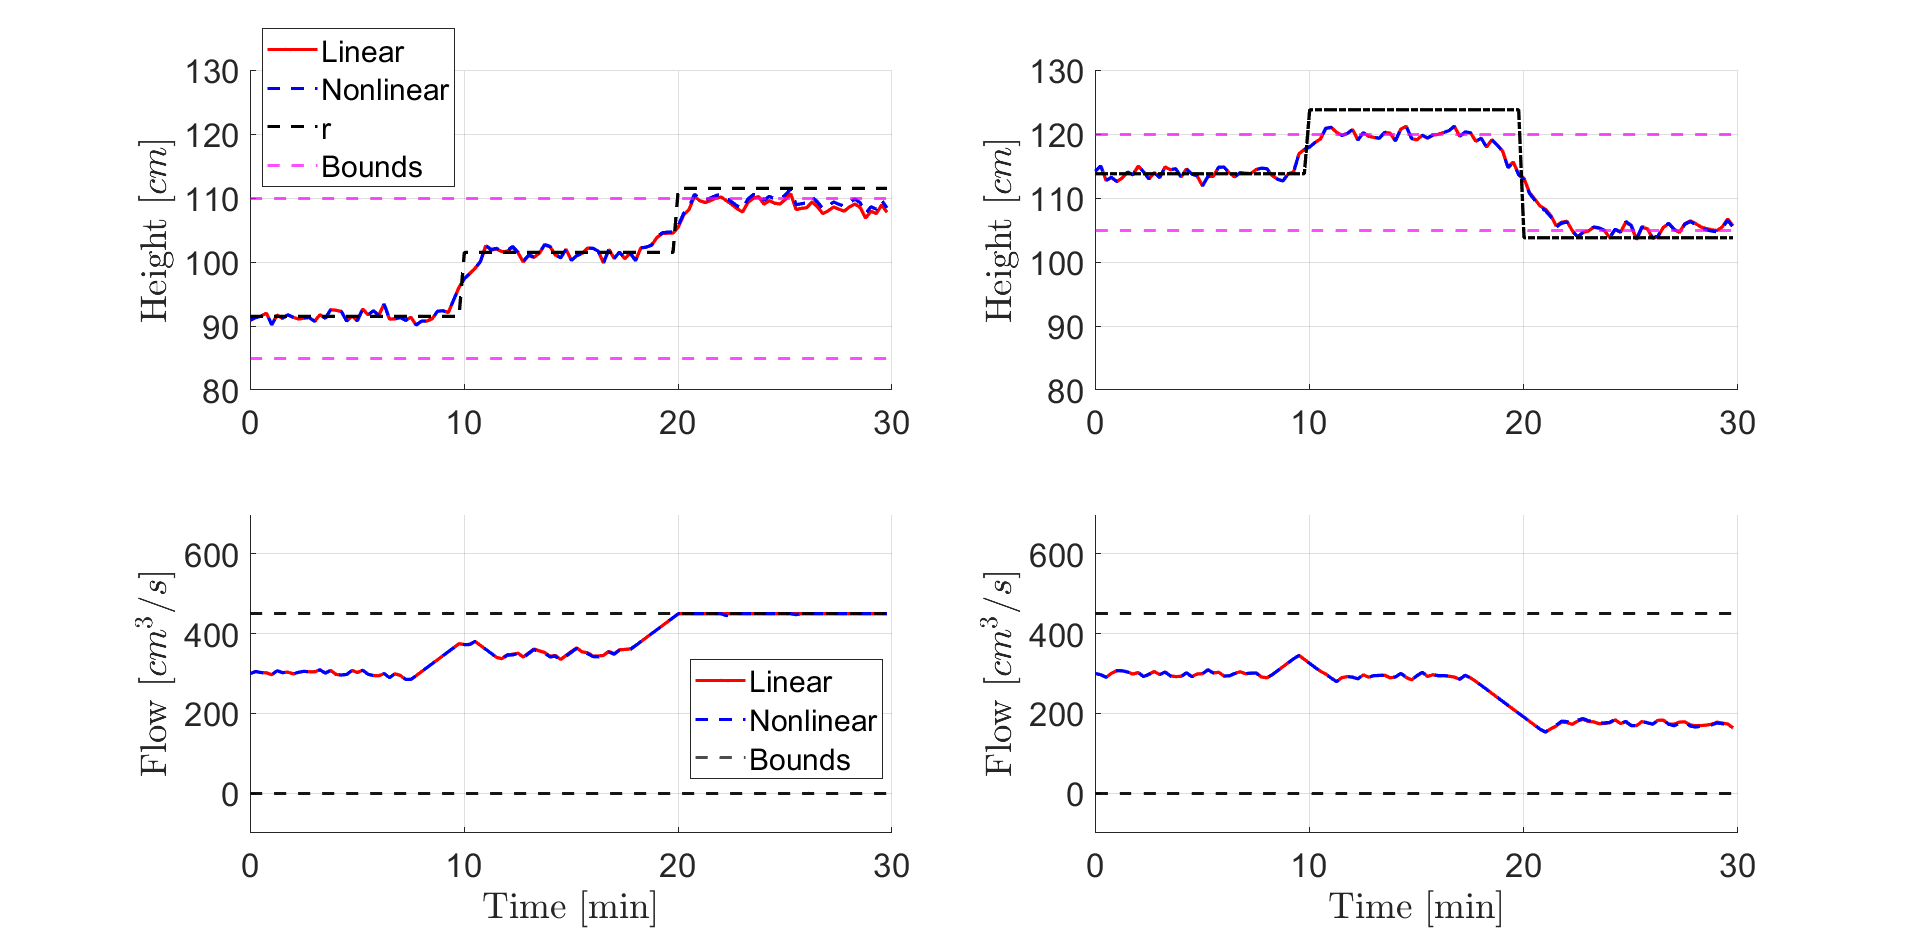
\includegraphics[width=1\textwidth]{Figures/Pr10.3_InOut_con_MPC.png}
    \caption{Input constrained output constrained MPC - Simulation on linear and non-linear model}
    %\label{fig:Kalman_stoc_state_step}
\end{figure}
By first analyzing the output in tank 1, it is seen that at $T=20\,[min]$ the reference changes. The system is both limited by the input which is a hard constraint, and therefore the system is not able to reach desired output. For tank 2, the input constraints are far from the operation, so these will not limit the system. The output constraint is clearly seen from $T=10-20\,[min]$ where the output is limited. The idea of a soft constraint is clearly seen since the controller allows system to trespass the value (which is caused by the present of noise). At $T=20\,[min]$ the reference changes again, and here the lower output constraint limits the output. Once again, the presence of noise is causing the output to become lower than the limit in some small periods. \\
Due to the structure of the system, the output constraint on e.g. tank 2 can also affect tank 1. If the water level reached the constraint, this will limit the flow input. But since the flow from the pump affects both tanks, the dynamics in tank 1 can be affected.